\scanpage{25}
\mspage{11}
is unique, and $g_i$ defined left multiplication by an arbitrary element of $L_i$, say $l_i^{\unsure{\alpha_i|\beta_i}}$ $(\alpha_i\in\hat{\mathbb Z})$. We pass from $u$ to $\operatorname{int}(g)\circ u$ by \inserted{keeping $p$, and by\unsure{,}} replacing the $g_i$ by the $gg_i$.

If $v$ is given by $q,(h_i)$, we have
\[
vu(l_i)=v(\operatorname{int}(g_i^{\unsure{\deleted{\unsure{-1}}|\unsure{-1}}})l_i^p)=\operatorname{int}(v(g_i^{\unsure{\deleted{\unsure{-1}}|\unsure{-1}}}))v(l_i)^p
\]
where
\[
v(l_i)=\operatorname{int}(h_i^{\unsure{\deleted{\unsure{-1}}|\unsure{-1}}})l_i^q\qquad\text{thus}\qquad v(l_i)^p=\operatorname{int}(h_i^{\unsure{\deleted{\unsure{-1}}|\unsure{-1}}})l_i^{pq}
\]
thus
\[
(23)\quad vu(l_i)=\operatorname{int}\bigl(\overset{\deleted{\unsure{(h_i v(g_i))^{-1}}}}{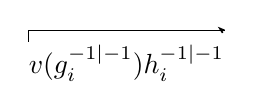
\begin{tikzpicture}[baseline=(prod.base)]
\node[inner sep=0pt] (prod) {$v(g_i^{\unsure{\deleted{\unsure{-1}}|\unsure{-1}}})h_i^{\unsure{\deleted{\unsure{-1}}|\unsure{-1}}}$};
\draw[line width=0.4pt] ([yshift=1pt]prod.north west) -- ([yshift=5pt]prod.north west) -- ([yshift=5pt]prod.north east);
\draw[line width=0.6pt] ([yshift=5pt]prod.north east) -- ++(-0.06,0.025) -- ++(0.035,-0.055);
\end{tikzpicture}}\bigr)l_i^{pq}
\]
If we denote by $S\overset{\unsure{\sim|\deleted{\sim}}}{\widehat{\widehat{\mathcal E}}}^!$ the extension of $\widehat{\widehat{\mathcal E}}^!$ by $\hat{\mathbb Z}^{\{0,1,\infty\}}$ defined \deleted{\unsure{by the pair|by the pairs|by the group}} \unsure{group|formed|formed} $\overset{\text{\begin{tikzpicture}[x=0.09cm,y=0.09cm,baseline=0ex]
\draw[line width=0.35pt] (0.45,0) .. controls (0.4,0.65) and (0.05,1.3) .. (0.02,1.05) .. controls (-0.05,0.65) and (0.5,0.35) .. (0.75,0.55) -- (1.15,1.1) -- (1.3,1.0);
\end{tikzpicture}}}{\text{of the}}$\unsure{.} \deleted{pairs} triples of a $u\in\widehat{\widehat{\mathcal E}}^!$ and of a system of $g_i$ which make explicit \inserted{via (21)} the isomorphism of the structure with loops ($p$ being the multiplier), we have on $S\overset{\unsure{\sim|\deleted{\sim}}}{\widehat{\widehat{\mathcal E}}}^!$ three functions with values in $\deleted{\unsure{\mathcal E}}\hat\Pi$
\[
(u,(g_i))\overset{\gamma_i}{\longmapsto}g_i,
\]
and we shall have\unsure{:}
\[
(24)\quad\gamma_i(\tilde v\tilde u)=\deleted{\unsure{\tilde v(\tilde u_i(\tilde u))\unsure{\cdot|:}\gamma_i(\tilde v)|\tilde v(\gamma_i(\tilde u))\unsure{\cdot|:}\gamma_i(\tilde v)}}\inserted{\deleted{\unsure{\gamma_i(\tilde v)\cdot v(\gamma_i(\tilde u))}} \tilde v(\gamma_i(\tilde u)\gamma_i\unsure{(}\tilde v)}
\]
i.e. $(\gamma_i)$ is a 1-cocycle on the group \deleted{$\unsure{\widehat{\widehat{\mathcal E}}^!}$}\inserted{$S\overset{\unsure{\sim|\deleted{\sim}}}{\widehat{\widehat{\mathcal E}}}^!$} with values in the group \deleted{\unsure{product of the group}}\inserted{opposite to the group} $\pi^{\{0,1,\infty\}}$.
\margin{\uline{NB} $S\widehat{\widehat{\mathcal E}}^!$ has been constructed as the group of Systems
\[
(p,g_0,g_1,g_\infty)\in\hat{\mathbb Z}^*\times\Pi^{[0,1,\infty]}
\]
satisfying the relation (22)}
\deleted{group}
The subgroup of $S\widehat{\widehat{\mathcal E}}^!$ kernel of $S\overset{\unsure{\sim|\deleted{\sim}}}{\widehat{\widehat{\mathcal E}}}\longrightarrow\operatorname{Aut}\operatorname{ext}_{\mathrm{lac}}^!(\widehat{\unsure{\pi|\Pi}})$ is identified with the product group
\[
\left(\hat\Pi\times\prod_{i\in\{0,1,\infty\}}L_i\right)\simeq\widehat{\unsure{\pi|\Pi}}\times\underset{\begin{tikzpicture}[x=0.10cm,y=0.10cm,baseline=0ex]
\draw[line width=0.3pt] (0,1.35) -- (0.25,0) -- (0.65,1.25);
\draw[line width=0.3pt] (1.05,1.15) -- (1.15,0.1);
\fill (1.0,1.65) circle (0.08);
\end{tikzpicture}}{\unsure{(\hat{\mathbb Z})^{\{0,1,\infty\}}|(\hat{\mathbb Z})^3}}
\]
\mspage{24}
